% Approfondimento di laboratorio di silmulazioni finanziarie in Latex
\documentclass[a4paper,11pt]{article}
\usepackage[T1]{fontenc}      % codifica dei font
\usepackage[utf8]{inputenc}
\usepackage[italian]{babel}
\usepackage{lipsum}
\usepackage{url}
\usepackage{package}
\usepackage{graphicx}
\begin{document}

\begin{frontespizio}
	\Universita{Paperopoli}
	\Logo{duck}
	\Facolta{Pennutologia}
	\Corso{Belle Lettere}
	\Annoaccademico{2030--2031}
	\Titoletto{Tesi di laurea magistrale}
	\Titolo{La mia tesi:\\ una lunga serie di risultati\\
		difficilissimi e complicatissimi}
	\Sottotitolo{Alcune considerazioni mutevoli}
	\Candidato[PP999999]{Paperon de’ Paperoni}
	\Relatore{Giovanni Episcopo}
	\Relatore{Pippo Cluvio}
\Correlatore{Ugo Frogio}
\Correlatore{Ubaldo Kutuzu}
\end{frontespizio}
\author{Erik Holler \and Elia Scarparo \and Stefano Zampiero}
\title{Approccio attuariale alla misurazione del rischio operativo}

\maketitle
\begin{abstract}
Descrizione dell'approccio attuariale alla misurazione del rischio operativo utilizzando come metodo il loss distribution approach
\end{abstract}
\tableofcontents

\section{RISCHIO OPERATIVO: DEFINIZIONE}
 Il Comitato di Basilea definisce il rischio operativo come \textit{corsivo}rischio di perdite dovute a inadeguati processi interni, errori umani, carenze nei sistemi operativi o a causa di eventi esterni. Working paper settembre 2001 –  Comitato di Basilea. Lo stesso Comitato prevede anche che: ogni banca, nel quadro di una visione integrata e coordinata del risk management, debba maturare una definizione interna di rischi operativi, in funzione del proprio business e dei propri requisiti organizzativi.\\
 Il concetto di rischio operativo è dunque intrinseco allo svolgimento di qualsiasi attività umana e per questo correlato ad ogni attività aziendale. Nell’ultimo decennio il sistema bancario e assicurativo è stato interessato da una consapevolezza crescente in merito alla portata strategica dell’attività di gestione e controllo dell’esposizione ai diversi tipi di rischio operativo. Tra i principali fattori che hanno portato a tale consapevolezza devono essere citati: crescita dimensionale delle banche, operazioni di fusione e acquisizione fra banche, massicci investimenti tecnologici attuati da banche, innovazione finanziaria che ha accresciuto la dipendenza da complesse procedure di calcolo e valutazione, sviluppo dei canali telematici, outsourcing. \\
È interessante osservare come sia diffusa l’idea che le perdite operative riguardino prevalentemente aree di business come l’investment banking o il trading su derivati, quando in realtà si riscontrano numerosi esempi di perdite che interessano anche le aree di business più tradizionali. \\
Comportamenti infedeli dei dipendenti, business practice improprie, disfunzioni nei sistemi di controllo interno, scarsa trasparenza nella prestazione dei servizi di investimento, sistemi premianti distorti e linee di reporting non chiare sono le evidenze emerse in dissesti finanziari clamorosi, da cui tutti hanno appreso quanto sia importante rafforzare i presidi sul rischio operativo specie in ambito finance e di seguire l’evoluzione di indicatori, anche non finanziari, sull’andamento dell’esposizione al rischio. \\
L’emanazione del “Nuovo Accordo sulla Convergenza Internazionale della Misurazione del Capitale e dei coefficienti Patrimoniali”, comunemente detto “Basilea II”, ha fatto in modo che il rischio operativo fosse opportunamente identificato, misurato e monitorato a presidio della solvibilità dell’azienda, con modelli di misurazione del rischio sempre più vicini alle specificità della stessa. È con Basilea 2 che viene esplicitata una definizione in positivo, la circolare n.263 
\subsection{Un sottoparagrafo}
\lipsum[1]
\begin{figure}[htbp]
	\centering
	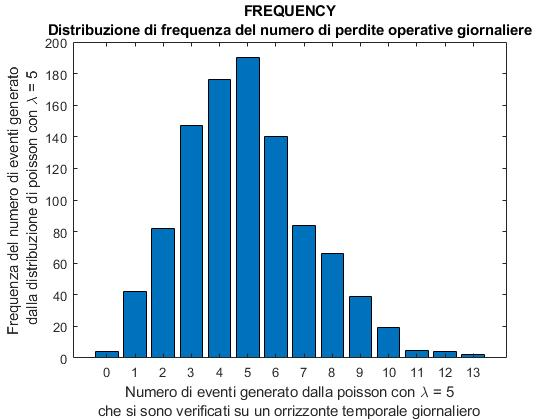
\includegraphics[width= 10cm]{FREQUENCY.jpg}
	\caption{frequency}
	\label{figuraaa}
\end{figure}
nella figura ~\ref{frequency}
\section{Un paragrafo}
\label{sec:esempio}
\lipsum[1]
% Bibliografia
\begin{thebibliography}{9}
\bibitem{pantieri:arte}
Pantieri, Lorenzo e Tommaso Gordini (2017),
\emph{L’arte di scrivere con \LaTeX},
\url{http://www.lorenzopantieri.net/LaTeX_files/ArteLaTeX.pdf}.
\end{thebibliography}
\end{document}